\chapter{Funciones de Legendre}

Como vimos anteriormente en el capítulo \ref{chap:MSV}, al resolver la ecuación de Helmholtz en coordenadas esféricas, podemos obtener dos ecucaciones, según el valor de la constante de separación $m^2$. 

\section{Ecuación y Funciones de Legendre}

Analizaremos en primer lugar el caso en que $m=0$, donde luego del cambio de variables $x = \cos \theta$, obtuvimos la EDO
% \begin{equation}
%     \frac{1}{\sin\theta} \frac{d}{d\theta}\left( \sin\theta \frac{d\Theta}{d\theta} \right) + \lambda \Theta = 0 \ ,
% \end{equation}
% que al considerar el cambio de variables $x = \cos\theta$, y llamar a $\Theta(\theta) = \Theta(\arccos(x)) = y(x)$, de modo que
% \begin{equation}
%     \frac{d}{d\theta} = \frac{dx}{d\theta} \frac{d}{dx} = -\sin\theta \frac{d}{dx} \ ,
% \end{equation}
% con lo que podremos escribir la ecuación como
\begin{equation}
    % \frac{1}{\sin\theta}(-\sin\theta)\frac{d}{dx}\left( \sin\theta (-\sin\theta) \frac{dy}{dx} \right) + \lambda y = 
    \frac{d}{dx}\left( (1-x^2) \frac{dy}{dx} \right) + \lambda y = 0 \ ,
\end{equation}
expresión que nombraremos como \textbf{ecuación de Legendre}, y que también puede ser escrita de forma más explícita como
\begin{equation}\label{eq:legendre_explicit}
    (1-x^2)\frac{d^2y}{dx^2} - 2x \frac{dy}{dx} + \lambda y = 0 \ .
\end{equation}

% Observamos que hemos escrito la ecuación de Legendre en la forma de una ecuación de Sturm-Liouville, con $p(x) = 1-x^2$ y $q(x) = r(x) = 1$. Observamos que,
Dado que $x=\cos\theta$, nuestra ecuación, y por ello sus soluciones, están definidas en el intervalo $[-1,1]$. Nos interesa que estos casos extremos posean soluciones finitas, lo que nos permitirá encontrar el valor de $\lambda$ para esta ecuación.

\subsection{Resolviendo la ecuación de Legendre}

% En primer lugar, escribimos la ecuación de forma más explícita, es decir,
% \begin{equation}\label{eq:legendre_explicit}
%     (1-x^2)y''(x) - 2x y'(x) + \lambda y(x) = 0 \ .
% \end{equation}

Utilizando el método de series, observamos que $P(x) = -2x/(1-x^2)$, y que $Q(x) = \lambda/(1-x^2)$. Ambas expresiones tienen puntos singulares en $x = \pm 1$, pero $x=0$ es un punto ordinario. Por ello, planteamos soluciones de la forma
\begin{equation}
    % \begin{dcases}
        y(x) = \sum_{k=0}^{\infty} a_k x^k \ ,
        %  \\
    %     y'(x) & = \sum_{k=1}^{\infty} k a_k x^{k-1} \\
    %     y''(x) & = \sum_{k=2}^{\infty} (k-1)k a_k x^{k-2} \\
    %     & = \sum_{k=0}^{\infty} (k+1) (k+2) a_{k-2} x^k 
    % \end{dcases} \ ,
\end{equation}
de modo que sustituyendo en la expresión \eqref{eq:legendre_explicit} tenemos 
\begin{align*}
    \sum_{k=0}^{\infty} (k+1)(k+2) a_{k+2} x^k - \sum_{k=0}^{\infty} (k-1) k a_k x^k - 2 \sum_{k=1}^{\infty} k a_k x^k + \lambda \sum_{k=0}^{\infty} a_k x^k & = 0 \ , \\
    \sum_{k=0}^{\infty} \left[ (k+1)(k+2) a_{k+2} - k(k-1)a_k  - 2k a_k + \lambda a_k \right]x^k & = 0 \ ,
\end{align*}
donde hemos usado que $\sum_{k=0}^{\infty} k = 0 + \sum_{k=1}^{\infty} k$. Dado que $x^k = 0$ corresponde a la solución trivial, analizamos la relación entre los coeficientes de nuestra ecuación,
\begin{equation}
    (k+1)(k+2) a_{k+2} - [(k-1) k + 2k - \lambda]a_k = 0 \ ,
\end{equation}
de donde encontramos la siguiente relación de recurrencia,
\begin{equation}\label{eq:recurrencia_legendre}
    a_{k+2} = \frac{k(k+1) - \lambda}{(k+1)(k+2)}a_k \ ,
\end{equation}
de modo que dados unos valores para $a_0$ y $a_1$ podremos determinar todos los coeficientes de nuestra expresión. Luego, si desarrollamos los términos pares e impares por separado, podemos observar la siguiente recurrencia,
\begin{align*}
    a_2 & = \frac{-\lambda}{2} a_0 \\
    a_4 & = \frac{2(2+1) - \lambda}{3 \cdot 4} a_2 = \frac{-\lambda(2(2+1)-\lambda)}{4!}a_0 \\
    a_6 & = \frac{4(4+1) - \lambda}{5 \cdot 6} a_4 = \frac{-\lambda (2(2+1)-\lambda)(4(4+1)-\lambda)}{6!} a_0 \\
    & \qquad \vdots \\
    a_n & = \frac{a_0}{n!}\prod_{\substack{\ell=0 \\ \ell \mbox{ \scriptsize{par}}}}^{n-2}[\ell (\ell+1) - \lambda] \ ,
\end{align*}
mientras que para el caso de coeficientes impares,
\begin{align*}
    a_3 & = \frac{1(1+1) - \lambda}{2 \cdot 3}a_1 \\
    a_5 & = \frac{(3(3+1)-\lambda)}{4 \cdot 5}a_3 = \frac{(1(1+1) - \lambda)(3(3+1)-\lambda)}{5!} a_1 \\
    a_7 & = \frac{5(5+1) - \lambda}{6 \cdot 7} = \frac{(1(1+1) - \lambda)(3(3+1)-\lambda)(5(5+1) - \lambda)}{7!} a_1 \\
    & \qquad \vdots \\
    a_n & = \frac{a_1}{n!}\prod_{\substack{\ell=1 \\ \ell \mbox{ \scriptsize{impar}}}}^{n-2}[\ell (\ell+1) - \lambda] \ ,
\end{align*}
de modo que la solución general para la ecuación de Legendre será la combinación lineal de la solución para los valores pares y la solución para los valores impares,
\begin{align}
    y(x) & = a_0 y_{1}(x) + a_1 y_{2}(x) \nonumber \\
    & = a_0 \left( \sum_{m=0}^{\infty} b_{m} x^{2m} \right) + a_1 \left( \sum_{m=0}^{\infty} c_{m} x^{2m+1} \right) \nonumber \\
    & = \sum_{m=0}^{\infty} \frac{a_0}{(2m)!}\left( \prod_{\substack{\ell=0 \\ \ell \mbox{ \scriptsize{par}}}}^{2m-2}[\ell (\ell+1) - \lambda] \right)x^{2m} + \sum_{m=0}^{\infty} \frac{a_1}{(2m+1)!}\left( \prod_{\substack{\ell=1 \\ \ell \mbox{ \scriptsize{impar}}}}^{2m-1}[\ell (\ell+1) - \lambda] \right)x^{2m+1} \ . \label{eq:Legendre_series_solution}
\end{align}

Con esto, podemos darnos cuenta de que la solución general de la ecuación de Legendre es una serie infinita, para la cual debemos analizar su convergencia en el intervalo $x \in [-1,1]$.

Según el criterio de la razón\footnote{Véase el capítulo 7 de \cite{Barea}}, la serie converge para $|x|<1$, independientemente del valor de $\lambda$. Nos queda analizar los casos extremos, es decir, $x= \pm 1$.

Para $\lambda \neq n(n+1)$, la serie diverge, puesto que ella se convierte en una serie numérica sin ningún tipo de restricción, que crece indefinidamente. Volveremos a este caso más tarde.

Para $\lambda = n (n+1)$, existirá algún término $a_n=0$ para una de las soluciones, la solución par $y_1(x)$ o la solución impar $y_2(x)$, tal que gracias a la relación de recurrencia \eqref{eq:recurrencia_legendre}, todo término superior a este se anulará. Luego, basta imponer que el primer coeficiente de la solución de paridad opuesta se anule para así obtener una solución convergente. Es decir, si $n$ es par, $a_1=0$, mientras que si $n$ es impar, escogemos $a_0 = 0$.

De esta forma, nos gustaría poder escribir una expresión general para las soluciones que son válidas en todo el dominio, es decir, cuando $\lambda = n(n+1)$. Notamos que $\ell(\ell+1)-n(n+1) = (\ell - n)(\ell + n + 1)$, podemos encontrar que, como una serie de potencias,
\begin{align} 
    y_{1,n}(x) & = \sum_{m=0}^{n/2} b_m x^{2m} = \sum_{m=0}^{n/2} \left(\frac{1}{(2m)!} \prod_{\substack{\ell=0 \\ \ell \mbox{ \scriptsize{par}}}}^{2m-2} (\ell-n)(\ell+n+1) \right) x^{2m} \\
    y_{2,n}(x) & = \sum_{m=0}^{(n-1)/2} c_m x^{2m+1} = \sum_{m=0}^{n/2} \left(\frac{1}{(2m)!} \prod_{\substack{\ell=1 \\ \ell \mbox{ \scriptsize{impar}}}}^{2m-2} (\ell-n)(\ell+n+1) \right) x^{2m+1}
\end{align}
o bien, mediante una expansión en términos de un conjunto de funciones $P_n(x)$,
\begin{align}
   y_{1,n}(x) & = d_{n,1} P_n(x) = \frac{(-1)^{n/2} 2^n \left[ \left(\frac{n}{2}\right)! \right]^2}{n!}P_n(x) \ , \label{eq:y1n_legendre}  \\
   y_{2,n}(x) & = d_{n,2} P_n(x) = \frac{(-1)^{(n+1)/2} 2^{n-1} \left[ \left(\frac{n-1}{2}\right)! \right]^2}{n!}P_n(x) \ . \label{eq:y2n_legendre}
\end{align}
% donde en ambos casos las funciones $P_n(x)$ corresponden a los \textbf{polinomios de Legendre}.


\begin{defi}\marginnote{Polinomios de Legendre}
    Los \textbf{Polinomios de Legendre de orden} $n$ corresponden a soluciones de la EDO de Legendre \eqref{eq:legendre_explicit}, que pueden ser definidas a partir de una serie de potencias como
    \begin{equation}
        P_n(x) = \sum_{k=0}^{n/2} \frac{(-1)^k (2n-2k)}{2^n k! (n-k)! (n-2k)!}x^{n-2k} \ .
    \end{equation}
    También pueden ser definidos a partir de la \emph{fórmula de Rodrigues}, según la cual pueden expresarse como
    \begin{equation}
        P_n(x) = \frac{1}{2^n n!} \frac{d^n}{dx^n} (x^2-1)^n \ .
    \end{equation}
\end{defi}
% definidos como

% Otra forma de definirlos es a partir 

En la figura \ref{fig:Legendre}, puede encontrar las gráficas de los primeros seis polinomios de Legendre, los que corresponden a

\begin{minipage}[b]{.45\textwidth}
    \begin{align*}
        P_0(x) & = 1 \ , \phantom{\frac{1}{2}} \\
        P_1(x) & = x \ , \phantom{\frac{1}{2}} \\
        P_2(x) & = \frac{1}{2}(3x^2 - 1) \ ,
    \end{align*}
\end{minipage}
\hfill
\begin{minipage}[b]{.45\textwidth}
    \begin{align*}
        P_3(x) & = \frac{1}{2}(5x^3 - 3x) \ , \\
        P_4(x) & = \frac{1}{8}(35x^4 - 15x^2 + 3) \ , \\
        P_5(x) & = \frac{1}{8}(63x^5 - 70x^3 + 15x) \ . 
    \end{align*}
\end{minipage}
% \begin{align*}
%     P_0(x) & = 1 \ , \\
%     P_1(x) & = x \ , \\
%     P_2(x) & = \frac{1}{2}(3x^2 - 1) \ , \\
%     P_3(x) & = \frac{1}{2}(5x^3 - 3x) \ , \\
%     P_4(x) & = \frac{1}{8}(35x^4 - 15x^2 + 3) \ , \\
%     P_5(x) & = \frac{1}{8}(63x^5 - 70x^3 + 15x) \ . 
% \end{align*}

\begin{figure}[htbp]
    \centering
    \includegraphics[width=12cm]{./Figuras/Legendre-Polynomials.pdf}
    \caption{Primeros seis polinomios de Legendre. Adaptación de \href{https://github.com/gfrubi/FM2/blob/master/figuras-editables/fig-Legendre.py}{este} código. La adaptación se encuentra \href{https://github.com/Pedroga-cc/Fisica-Matematica-II/blob/main/Figuras/Plotter_Legendre.py}{aquí}.}
    \label{fig:Legendre}
\end{figure}

\subsection{Función Generatriz}

\begin{defi}\marginnote{Función Generatriz}
    Para cualquier conjunto de \emph{polinomios ortogonales} $\{P_n(x)\}_{n\in \mathbb{N}}$, se denomina \textbf{función generatriz} (o generadora) de dicho conjunto a la función $G(x,t)$, tal que al ser desarrollada en una serie de Taylor para $t$, los coeficientes de dicha expansión son los polinomios $P_n(x)$:
\begin{equation}
    G(x,t) = \sum_{n=0}^{\infty} P_n(x)t^n \ .
\end{equation}
\end{defi}

En particular, la función generatriz para los polinomios de Legendre es dada por la expresión
\begin{equation}
    G(x,t) = \frac{1}{\sqrt{1-2xt + t^2}} \ .
\end{equation}
Si observamos esta expresión en detalle, y hacemos $t=r/a$ y $x = \cos\theta$, podemos escribir la función generatriz como
\begin{equation}
    G(\theta, r) = \frac{1}{\sqrt{1-2r \cos(\theta)/a + r^2/a^2}} = \frac{a}{\sqrt{a^2-2ar\cos\theta + r^2}} = \frac{a}{|\vec{x}-\vec{a}|} \ , 
\end{equation} 
donde $|\vec{x}-\vec{a}|$ es la distancia entre los puntos $\vec{x}$ y $\vec{a}$. Así, obtenemos la relación entre la distancia entre dos puntos del espacio con los Polinomios de Legendre,
\begin{equation} \label{eq:Legendre_distancias}
    \frac{1}{|\vec{x} - \vec{a}|} = \frac{1}{a}\sum_{\ell=0}^\infty \left( \frac{r}{a} \right)^\ell P_\ell(\cos\theta) \ .
\end{equation} 
En esta expresión, hemos asumido que $r>a$. En caso contrario, deben invertirse las relaciones dentro de la suma, ubicando $r$ en el lugar de $a$, y viceversa.

\begin{ejemplo}
    Expanda la expresión para un potencial electrostático generado por una carga puntual $q$ en la posición $\vec{a}$ en la región $r < a$.

    \textbf{Solución.} Recordamos que el potencial electrostático debido a una carga puntual es dado por
    \begin{equation}
        \phi(\x) = \frac{1}{4\pi \epsilon_0} \frac{q}{|\x - \vec{a}|} \ .
    \end{equation}

    Reemplazando el resultado obtenido en \eqref{eq:Legendre_distancias}, tenemos que
    \begin{equation}
        \phi(\vec{r}) = \frac{q}{4\pi \epsilon_0 r} \sum_{\ell=0}^\infty \left( \frac{a}{r} \right)^\ell P_\ell(\cos\theta) \ .
    \end{equation}

    La importancia de este resultado es que es la base de la llamada \emph{expansión multipolar}, que estudiarán detalladamente en su curso de electrodinámica.
\end{ejemplo}

% Podemos utilizar este resultado, por ejemplo, para escribir el potencial electrostático en un punto $\vec{r}$ producido por una carga $q$ en el punto $\vec{a}$,

% lo que se asocia a la llamada \emph{expansión multipolar}, que estudiarán en su curso de electrodinámica.

A partir de su función generadora, podemos encontrar explícitamente los polinomios de Legendre mediante la relación
\begin{equation}
    P_n(x) = \frac{1}{n!} \left[ \frac{\partial ^n G(t,x)}{\partial t^n}  \right]_{t=0} \ .
\end{equation}

\subsection{Propiedades}

\begin{propiedad}
    \textbf{Propiedades de los polinomios de Legendre.}

    \begin{enumerate}
        \item \textbf{Normalización.} Los polinomios de Legendre son funciones normalizadas, de modo que $P_n(1) = 1$, para cualquier valor de $n$.
        \item \textbf{Paridad.} Podemos encontrar que los polinomios de Legendre pueden ser funciones pares o impares según el valor de $n$, ya que
        \begin{equation}
            P_n(-x) = (-1)^n P_n(x) \ . 
        \end{equation}
    
        \item \textbf{Valor en el origen.} A partir de la función generatriz, podemos mostrar que
        % propiedad de paridad, podemos observar que, como los polinomios son \emph{impares} para $n$ impar, deberá cumplirse que $P_n(0) = 0$, para $n$ impar. Por otro lado, utilizando la función generatriz, podemos obtener que si $n$ es par, entonces
        \begin{equation}
            P_n(0) = \begin{dcases}
                0 \ , \qquad \text{si } n \text{ es impar.} \\
                (-1)^{n/2} \frac{n!}{2^n ((n/2)!)^2} \ , \qquad \text{si } n \text{ es par.}
            \end{dcases}
        \end{equation}
    
        \item \textbf{Ortogonalidad.} Los polinomios de Legendre satisfacen la relación de ortogonalidad
        \begin{equation}
            \int\limits_{-1}^1 P_n(x) P_m(x) dx = \frac{2}{2n+1} \delta_{n,m} \ .
        \end{equation}
    
        \item \textbf{Completitud.} Los polinomios de Legendre forman un \emph{conjunto completo} de funciones definidas en $[-1,1]$, por lo que forma una base para dichas funciones, lo que se expresa como
        \begin{equation}
            \sum_{n=0}^\infty \frac{2n+1}{2} P_n(x) P_n(x') = \delta(x-x') \ .
        \end{equation}
    
        \item \textbf{Serie de Fourier-Legendre.} Dado que los polinomios de Legendre forman una base en el intervalo $[-1,1]$, podemos expandir cualquier función en una Serie de Fourier-Legendre, tal que
    
        \begin{equation}
            f(x) = \sum_{n=0}^\infty a_n P_n(x) \ ,
        \end{equation}
        donde 
        \begin{equation}
            a_n = \frac{2n+1}{2} \int_{-1}^1 f(x) P_n(x) dx \ .
        \end{equation}
         
        \item \textbf{Relaciones de recurrencia.} Los polinomios de Legendre satisfacen las siguientes relaciones de recurrencia,
        \begin{align}
            n P_{n-1}(x) + (n+1) P_{n+1}(x) & = (2n+1) x P_n(x) \ , \\
            (2n+1) P_n(x) & = P'_{n+1}(x) - P'_{n-1}(x) \ .
        \end{align}    
    \end{enumerate}
\end{propiedad}

\begin{ejemplo}
    \textbf{(Arfken 15.2.2.)} Considere una esfera conductora sin carga de radio $r_0$ que es ubicada en un campo eléctrico uniforme de magnitud $E_0$, como se observa en la figura. Encuentre el nuevo potencial electrostático, perturbado por la ubicación de la esfera, y que satisface la ecuación de Laplace $\nabla^2 \psi = 0$.    

    \begin{center}
    \includegraphics[width = 6cm]{Figuras/Ejemplo-esfera-conductora-2.png}
    \end{center}

    \textbf{Solución.} Trabajaremos en coordenadas esféricas con el origen en el centro de la esfera y el eje $z$ orientado paralelamente al campo uniforme original. Recordemos que el potencial electrostático es una función \emph{continua}, de modo que en la frontera entre el interior y el exterior de la esfera (es decir, en $r = r_0$) la función potencial interior deberá tener el mismo valor que la función potencial exterior.
    
    Dado que la esfera es conductora, esta es \emph{equipotencial}, lo que significa que el potencial es el mismo en todo su volumen, tal que $\psi(r \leq r_0) = V_0$. En particular, dado que la esfera no está cargada, $V_0 = 0$. Supondremos también que en el plano $\theta = \pi/2$, $V = 0$. Esta será nuestra primera condición de borde.

    Separando variables, obtendremos una ecuación radial con soluciones $a_\ell r^\ell + b_\ell r^{-\ell-1}$, y una ecuación axial que corresponde a la ecuación de Legendre. Dada la simetría esférica del sistema, se ha asumido que $m=0$, de modo que la ecuación azimutal da origen a una constante. De este modo, nuestro potencial tendrá la forma
    \begin{equation*}
        \psi(r, \theta) = \sum_{\ell = 0}^\infty \left( a_\ell r^\ell + b_\ell r^{-\ell-1} \right) P_\ell(\cos \theta) \ , \quad r > r_0 \ .
    \end{equation*}

    El efecto de insertar la esfera en el campo eléctrico es local, por lo que el potencial electrostático \emph{muy lejos} de la esfera deberá comportarse como si el campo siguiera siendo uniforme,
    \begin{equation*}
        \psi(r \to \infty, \theta) = - E_0 z = -E_0 r \cos \theta = - E_0 r P_1(\cos \theta) \ ,
    \end{equation*}
    que será nuestra segunda condición de borde. Esta corresponde al caso en que nuestra serie satisface
    \begin{equation*}
        a_1 = -E_0 \ , \qquad a_n = 0 \ , n > 1 \ .
    \end{equation*}

    ¿Por qué es relevante esta elección? Si considerásemos que, por ejemplo, $a_2 \neq 0$, tendríamos términos cuadráticos que dominarían el comportamiento del potencial, de modo que la segunda condición de borde no se estaría satisfaciendo.

    Volviendo a nuestra primera condición de borde, estudiemos el comportamiento de la función en $r = r_0$ y $\theta = \pi/2$. tendremos
    \begin{equation*}
        \psi(r = r_0, \theta = \pi/2) = \frac{b_0}{r_0} + \left( \frac{b_1}{r_0^2} - E_0 r_0 \right) P_1 (\cos \theta) + \sum_{\ell=2}^\infty b_\ell \frac{P_\ell (\cos \theta)}{r_0^{\ell+1}} = 0 \ .
    \end{equation*}

    Esta igualdad se satisface si $b_n = 0$ para $n > 2$. Dado que la esfera no se encuentra cargada, $b_0 = 0$. Por último, despejando $b_1$, encontramos que su valor es
    \begin{equation*}
        b_1 = E_0 r_0^3 \ .
    \end{equation*}

    Así, el potencial electrostático en el exterior de la esfera tendrá la forma
    \begin{equation*}
        \psi_{\text{ext}}(r, \theta) = -E_0 r P_1(\cos \theta) + \frac{E_0 r_0^3}{r^2} P_1(\cos\theta) = - E_0 r \left(1 - \frac{r_0^3}{r^3} \right) P_1 (\cos \theta) \ .
    \end{equation*}

\end{ejemplo}

\subsection{Funciones de Legendre de segunda especie}

Como discutimos anteriormente, al escoger $\lambda = n(n+1)$ para un número entero $n$, debemos truncar una de las series que aparecen en la ecuación \eqref{eq:Legendre_series_solution}, de modo que la solución se reduce a los polinomios de Legendre. El motivo de hacer esto es hallar una solución que converja en $x = \pm 1$. Sin embargo, ¿debemos hacer esto si nuestro problema no requiere convergencia en los contornos $x = \pm 1$?

\begin{defi}\marginnote{Funciones de Legendre de segunda especie}
    Las soluciones a la ecuación de Legendre \eqref{eq:legendre_explicit} que no son convergentes en los puntos $x = \pm 1$ son llamadas \textbf{funciones de Legendre de segunda especie}, denotadas por $Q_n(x)$. Estas se definen como
    \begin{align} \label{eq:legendre-second-kind}
        Q_n(x) & = \begin{dcases}
            d_{1,n} y_{2,n}(x) \ , \qquad \text{ si } n \text{ es par} \ , \\
            d_{2,n} y_{1,n}(x) \ , \qquad \text{ si } n \text{ es impar} \ ,
        \end{dcases} \\
        & = \left\{ \begin{array}{cc}
            (-1)^{n/2} \dfrac{[(n/2)!]^2}{n!} 2^n y_{2,n}(x) , & \text{ si } n \text{ es par} \ , \\
            (-1)^{(n+1)/2} \dfrac{[\left((n-1)/2\right)!]^2}{n!} 2^{n-1} y_{1,n}(x) \ , & \text{ si } n \text{ es impar} \ ,
        \end{array} \right.
    \end{align}
    donde $y_{1,n}$ e $y_{2,n}$ son las funciones definidas en \eqref{eq:y1n_legendre} y \eqref{eq:y2n_legendre}, respectivamente. 
    
    Nótese que \emph{a la solución para} $n$ \emph{par, hemos multiplicado los coeficientes de la solución impar}, y viceversa.
\end{defi}

% La respuesta es no, y de hecho ciertos problemas físicos requieren de estas soluciones. Por ello, las llamaremos \textbf{funciones de Legendre de segunda especie}, denotadas por $Q_n(x)$, y que definimos como
% \begin{align}
%     Q_n(x) & = \begin{dcases}
%         d_{1,n} y_{2,n}(x) \ , \qquad \text{ si } n \text{ es par} \ , \\
%         d_{2,n} y_{1,n}(x) \ , \qquad \text{ si } n \text{ es impar} \ ,
%     \end{dcases} \\
%     & = \begin{dcases}
%         (-1)^{n/2} \frac{[(n/2)!]^2}{n!} 2^n y_{2,n}(x) \ , \qquad \text{ si } n \text{ es par} \ , \\
%         (-1)^{(n+1)/2} \frac{[\left(\frac{n-1}{2}\right)!]^2}{n!} 2^{n-1} y_{1,n}(x) \ , \qquad \text{ si } n \text{ es impar} \ ,
%     \end{dcases}
% \end{align}
% donde $y_{1,n}$ e $y_{2,n}$ son las funciones definidas en \eqref{eq:y1n_legendre} y \eqref{eq:y2n_legendre}, respectivamente. Nótese que \emph{a la solución para} $n$ \emph{par, hemos multiplicado los coeficientes de la solución impar}, y viceversa.

Las funciones asociadas de Legendre satisfacen las mismas relaciones de recurrencia que las funciones de Legendre, de modo que
\begin{align}
    nQ_{n-1}(x) + (n+1)Q_{n+1}(x) & = (2n+1) x Q_n(x) \ , \\
    (2n+1)Q_n(x) & = Q'_{n+1}(x) - Q'_{n-1}(x) \ . 
\end{align}
Gracias a ellas, podemos obtener las expresiones explícitas para funciones de orden superior, debiendo utilizar la definición \eqref{eq:legendre-second-kind} únicamente para las funciones $Q_0(x)$ y $Q_1(x)$. Pueden encontrar estas derivaciones en el capítulo 5 de \cite{Rubilar}.

Las primeras seis funciones de Legendre de segunda especie son graficadas en la figura \ref{fig:Legendre-second-kind}, y las expresiones para las primeras cuatro son dadas por

\begin{minipage}[b]{.45\textwidth}
    \begin{align*}
        Q_0(x) & = \frac{1}{2} \ln\left( \frac{1+x}{1-x} \right) \ , \\
        Q_1(x) & = \frac{x}{2} \ln\left( \frac{1+x}{1-x} \right) - 1 \ ,
    \end{align*}
\end{minipage}
\hfill
\begin{minipage}[b]{.5\textwidth}
    \begin{align*}
        Q_2(x) & = \frac{3x^2-1}{4}\ln\left( \frac{1+x}{1-x} \right) - \frac{3x}{2} \ , \\
        Q_3(x) & = \frac{5x^3 - 3x}{4}\ln\left( \frac{1+x}{1-x} \right) - \frac{5x^2}{2} + \frac{2}{3} \ . 
    \end{align*}
\end{minipage}

\begin{figure}[htbp]
    \centering
    \includegraphics[width=12cm]{Figuras/Legendre-second-kind.pdf}
    \caption{Primeras seis funciones de Legendre de segunda especie. Nótese el comportamiento asintótico alrededor de los extremos $x = -1$ y $x=1$. Adaptación de \href{https://github.com/gfrubi/FM2/blob/master/figuras-editables/fig-Legendre.py}{este} código. La adaptación se encuentra \href{https://github.com/Pedroga-cc/Fisica-Matematica-II/blob/main/Figuras/Plotter_Legendre.py}{aquí}.}
    \label{fig:Legendre-second-kind}
\end{figure}

\begin{propiedad}
    \textbf{Propiedades de las funciones de Legendre de segunda especie.}

    \begin{enumerate}
        \item \textbf{Paridad.} Se tiene que
        \begin{equation}
            Q_n(-x) = (-1)^{n+1} Q_n(x) \ .
        \end{equation}
        \item \textbf{Valor en el origen.} Dada su paridad, las relaciones se invierten respecto a los polinomios de Legendre, de modo que
        \begin{equation}
            Q_n(0) = \begin{dcases}
                0 \ , \qquad \text{si } n \text{ es par} \ , \\
                (-1)^{(n+1)/2} \frac{\left[ \left( \frac{n-1}{2} \right)! \right]^2}{n!} 2^{n-1} \ , \qquad \text{si } n \text{ es impar} \ .  
            \end{dcases}
        \end{equation}
        \item \textbf{Valor en el extremo del intervalo.} Los extremos del intervalo son puntos singulares para estas funciones, de modo que
        \begin{equation}
            \lim_{x \to 1} Q_n(x) = +\infty \ .
        \end{equation}
    \end{enumerate} 
\end{propiedad}

% Otras propiedades relebvantes que estas satisfacen son


En resumen, la solución general de la EDO de Legendre para $\lambda = n(n+1)$, es dada por
\begin{equation}
    y(x) = C_1 P_n(x) + C_2 Q_n(x) \ ,
\end{equation}
donde los polinomios de Legendre $P_n(x)$ convergen en todo el intervalo $[-1,1]$, incluídos los extremos, mientras que las funciones de segunda especie $Q_n(x)$ convergen en el interior del intervalo $(-1,1)$, mas no en los extremos.

\begin{obs}{Observación}
    Si bien lo más adecuado es plantear siempre la solución a la EDO de Legendre considerando las funciones de primera y segunda especie, la gran mayoría de problemas físicos descartarán la solución de segunda especie, dada su divergencia en los extremos.

    La referencia \cite{Lebedev_Silverman_1972} plantea que las funciones de segunda especie aparecerán en problemas poco comunes, como el campo electrostático en un conductor toroidal, o en la atracción gravitacional ejercida por un esferoide sólido, entre otras. Puede revisar el capítulo 8 de esa referencia para más detalles.
\end{obs}

\section{Ecuación y funciones asociadas de Legendre}

Hasta ahora, analizamos el caso en que $m=0$ en la EDO axial \eqref{eq:Helmholtz_esferica} que se obtiene de la ecuación de Helmholtz. En lo que resta del capítulo, analizaremos el caso en que $m \neq 0$.

En este caso, bajo el cambio de variable $x=\cos\theta$, la ecuación \eqref{eq:Helmholtz_esferica} toma la forma de la 
% \begin{equation}
%     \frac{1}{\sin\theta} \frac{d}{d\theta}\left( \sin\theta \frac{d\Theta}{d\theta} \right) + \left(\lambda - \frac{m^2}{\sin^2\theta} \right) \Theta = 0 \ .
% \end{equation}
%
% Realizando nuestro cambio de variable $x = \cos\theta$, y desarrollando de forma más explícita la ecuación, esta toma la forma de la 
\textbf{ecuación asociada de Legendre},
\begin{equation}\label{eq:EDO_asociada_Legendre}
    (1-x^2) \frac{d^2y}{dx^2} - 2x\frac{dy}{dx} + \left( \lambda - \frac{m^2}{1-x^2} \right) y = 0 \ ,
\end{equation}
cuyas soluciones se encuentran definidas en el intervalo $[-1,1]$.

\subsection{Resolviendo la ecuación asociada de Legendre}

Para hacer más fácil el proceso de utilizar el método de series, realizamos la sustitución $y(x) = (1-x^2)^{m/2} u(x)$, de modo que
\begin{align*}
    y'(x) & = \frac{\left(1 - x^{2}\right)^{\frac{m}{2}} \left((1 - x^2) u'\left(x\right) - mx u\left(x\right)\right)}{1 - x^2} \\
    %  -m x (1-x^2)^{m/2 - 1} u(x) + (1-x^2)^{m/2} u'(x) \\
    y''(x) & = \frac{\left(1 - x^{2}\right)^{\frac{m}{2}} \left[(1-x^2)^2 u'' \left(x\right) - 2mx (1 - x^2) u'(x) + m\left((m - 1) x^{2} - 1\right) u\left(x\right)\right]}{(1- x^2)^2} \ .
\end{align*}

Reemplazamos esta función y sus derivadas en \eqref{eq:EDO_asociada_Legendre}, de modo que
\begin{align*}
    (1-x^2)\frac{\left(1 - x^{2}\right)^{\frac{m}{2}} \left[(1-x^2)^2 u'' \left(x\right) - 2mx (1 - x^2) u'(x) + m\left((m - 1) x^{2} - 1\right) u\left(x\right)\right]}{(1- x^2)^2} & \\
    - 2x \frac{\left(1 - x^{2}\right)^{\frac{m}{2}} \left((1 - x^2) u'\left(x\right) - mx u\left(x\right)\right)}{1 - x^2} + \left(\lambda - \frac{m^2}{1-x^2}\right) (1-x^2)^{m/2} u(x) & = 0 \\
    % \frac{\left[(1-x^2)^2 u'' \left(x\right) - 2mx (1 - x^2) u'(x) + m\left((m - 1) x^{2} - 1\right) u\left(x\right)\right]}{(1- x^2)} - 2x & \\
    % \frac{\left((1 - x^2) u'\left(x\right) - mx u\left(x\right)\right)}{1 - x^2} + \left(\lambda - \frac{m^2}{1-x^2}\right) (1-x^2)^{m/2} u(x) + \left(\lambda - \frac{m^2}{1-x^2}\right) u(x) & = 0 \\
    (1-x^2) u''(x)  - 2m (x + 1) u'(x) + \left[ \left( \lambda - \frac{m^2}{1-x^2} \right) + \frac{2mx + m[(m-1)x^2 - 1]}{1-x^2} \right]u(x) & = 0 \\
    (1-x^2) u''(x)  - 2m (x + 1) u'(x) + \left[ \frac{\lambda(1-x^2) - m(m+1)(1-x^2)}{1-x^2} \right]u(x) & = 0 \,
\end{align*}
%
% \hrule
%
% AA
%
% \hrule
%
lo que resulta en la EDO para $u(x)$
\begin{equation}
    (1-x^2)u''(x) - 2x(m+1)u'(x) + (\lambda - m(m+1))u(x) = 0 \ .
\end{equation}

En este caso, $P(x) = 2x(m+1)/(1-x^2)$ y que $Q(x) = (\lambda - m(m+1))/(1-x^2)$, de modo que como ambas funciones son analíticas en $x=0$, podemos plantear una solución de la forma
\begin{equation}
    u(x) = \sum_{k=0}^{+\infty} a_k x^k 
\end{equation} 
que nos llevará a la relación de recurrencia
\begin{equation}\label{eq:recurrencia_asociadas}
    a_{k+2} = \frac{k^2 + (2m+1)k - \lambda + m(m+1)}{(k+1)(k+2)} a_k \ ,
\end{equation}
que al igual que para la ecuación de Legendre, resultará en series que convergen para $|x|<1$ y, en general, divergen para $|x|=1$, salvo para ciertos valores de $\lambda$. Para encontrar dichos valores, necesitamos que el numerador de la ecuación \eqref{eq:recurrencia_asociadas} sea cero. Esto impone que $\lambda$ debe satisfacer la igualdad
\begin{equation}
    \lambda = m(m+1) + k(k+1) + 2mk = (m+k)(m+k+1) \ ,
\end{equation}
y definiendo $n = m+k \geq m$, observamos que nuevamente requeriremos que $\lambda = n(n+1)$, de modo que la serie se truncará luego del $(n-m)$-ésimo término.

Podemos hallar de forma explícita las soluciones a esta EDO diferenciando repetidamente la ecuación de Legendre \eqref{eq:legendre_explicit}, al hacer uso de la regla de Leibniz, es decir,
\begin{equation}
    \frac{d^m}{dx^m}\left( f_1(x) \cdot f_2(x) \right) = \sum_{s=0}^{m} \binom{m}{s} \frac{d^{m-s}f_1(x)}{dx^{m-s}} \frac{d^s f_2(x)}{dx^s} \ ,
\end{equation}
de donde obtenemos que
\begin{align*}
    \frac{d^m}{dx^m}\left[ (1-x^2)y'' \right] & = \binom{m}{m} (1-x^2) \frac{d^m y''}{dx^m} - \binom{m}{m-1} 2x \frac{d^{m-1} y''}{dx^{m-1}}  - \binom{m}{m-2} 2 \frac{d^{m-2} y''}{dx^{m-2}} \\
    & = (1-x^2) \left(\frac{d^m y}{dx^m}\right)'' - 2mx \left(\frac{d^m y}{dx^m}\right)' - m(m-1)\left(\frac{d^m y}{dx^m}\right)  \\
    \frac{d^m}{dx^m}\left[ 2x y' \right] & = \binom{m}{m} 2x \frac{d^m y'}{dx^m} + \binom{m}{m-1} 2 \frac{d^{m-1} y'}{dx^{m-1}} \\
    & = 2x \left(\frac{d^2 y}{dx^2}\right)' + 2m \left(\frac{d^2 y}{dx^2}\right) \\
    \frac{d^m}{dx^m}\left[ n(n+1)y \right] & = n(n+1) \frac{d^m y}{dx^m} \ ,
\end{align*}
donde hemos usando que $\binom{m}{m} = 1$, $\binom{m}{m-1} = m$, y $\binom{m}{m-2} = \frac{m(m-1)}{2}$. Así, la EDO resulta en
\begin{align*}
    (1-x^2)\left(\frac{d^m y}{dx^m}\right)'' - (2mx + 2x) \left(\frac{d^m y}{dx^m}\right)' + [m(m-1) + 2m + n(n+1)]\left(\frac{d^m y}{dx^m}\right) & = 0 \\
    (1-x^2)\left(\frac{d^m y}{dx^m}\right)'' - 2x(m + 1) \left(\frac{d^m y}{dx^m}\right)' + [m(m+1) + n(n+1)]\left(\frac{d^m y}{dx^m}\right) & = 0 \ , 
\end{align*}
donde al hacer la sustitución $f(x) = y^{(m)}(x)$, obtenemos la EDO para $u(x)$ cuando $\lambda = n(n+1)$. De esta forma, concluímos que las funciones $u(x)$ deberán ser proporcionales a $\frac{d^m }{dx^m} P_n(x)$.

\begin{defi}\marginnote{Polinomios asociados de Legendre}
    Se definen los \textbf{polinomios asociados de Legendre}, soluciones de la EDO \eqref{eq:EDO_asociada_Legendre}, como
    \begin{equation} \label{eq:asociadas_legendre}
        P_n^m(x) = (1-x^2)^{m/2} \frac{d^m}{dx^m}P_n(x) \ ,
    \end{equation}
    donde el factor $(1-x^2)^{m/2}$ es introducido para una correcta normalización. Nótese que cuando $m=0$, se recuperan los polinomios de Legendre \eqref{eq:Legendre_series_solution}, de modo que $P_n^0(x) \equiv P_n(x)$. 

    También se admite la definición mediante la fórmula de Rodrigues
    \begin{equation} \label{eq:rodrigues-asociados}
        P_n^m(x) = \frac{1}{2^n n!}(1-x^2)^{m/2} \frac{d^{n+m}}{dx^{n+m}}(x^2-1)^n \ ,
    \end{equation}
    obtenida al sustituir la fórmula de Rodrigues para los polinomios de Legendre en la ecuación \eqref{eq:asociadas_legendre}, y es también válida para $m<0$, siempre y cuando $|m|\leq n$.
\end{defi}

% De forma convencional (por motivos de normalización), las soluciones $u(x)$ corresponden a los \textbf{polinomios asociadas de Legendre}, expresados como
% \begin{equation} \label{eq:asociadas_legendre}
%     P_n^m(x) = (1-x^2)^{m/2} \frac{d^m}{dx^m}P_n(x) \ .
% \end{equation}

% Observamos que cuando $m=0$, recuperamos los polinomios de Legendre, de modo que $P^0_n(x) \equiv P_n(x)$. Sustituyendo la fórmula de Rodrigues para $P_n(x)$ en \eqref{eq:asociadas_legendre}, obtenemos la \emph{fórmula de Rodrigues para los polinomios asociados de Legendre},
% \begin{equation} \label{eq:rodrigues-asociados}
%     P_n^m(x) = \frac{1}{2^n n!}(1-x^2)^{m/2} \frac{d^{n+m}}{dx^{n+m}}(x^2-1)^n \ ,
% \end{equation}
% que también es válida para $m<0$, siempre y cuando $|m|\leq n$.

\subsection{Función generatriz}

En este caso, podemos hacer uso de la relación entre los polinomios asociados de Legendre y los polinomios de Legendre para obtener la función generatriz de los primeros. En efecto, observamos que derivando $m$ veces la función generatriz de los polinomios de Legendre respecto a $x$, tenemos
\begin{equation}
    \frac{d^m G}{dx^m} = \frac{d^m}{dx^m}(1-2xt+t^2)^{-1/2} = \sum_{n=0}^\infty \frac{d^m}{dx^m}P_n(x) t^n \ ,
\end{equation}
y multiplicando ambos lados por $(1-x^2)^{m/2}$, tenemos que
\begin{equation}
    \frac{d^m G}{dx^m} = (1-x^2)^{m/2} \frac{d^m}{dx^m}(1-2xt+t^2)^{-1/2} = \sum_{n=0}^\infty P^m_n(x) t^n \ .
\end{equation}

Derivando el lado izquierdo de la ecuación, obtenemos
\begin{equation}
    \frac{1 \cdot 3 \cdot 5 \dots (2m-1) (1-x^2)^{m/2} t^m}{(1-2xt+t^2)^{m+1/2}} = \sum_{n=0}^\infty P_n^m t^n \ .
\end{equation}
Dividimos la expresión por $t^m$, definimos una variable auxiliar $r=n-m$, y además notamos que
\begin{equation}
    1 \cdot 3 \cdot 5 \dots (2r-1) = \frac{1 \cdot 2 \cdot 3 \dots 2r}{2 \cdot 4 \cdot 6 \dots 2r} = \frac{(2r)!}{2^r r!} \ .
\end{equation}

De este modo, podemos hallar que
\begin{equation}
    G_m(x,t) = \frac{(2m)! (1-x^2)^{m/2}}{2^m m! (1-2xt+t^2)^{m+1/2}} = \sum_{r=0}^\infty P_{r+m}^m(x) t^r \ .
\end{equation}

\subsection{Propiedades}

\begin{propiedad}
    \textbf{Propiedades de los polinomios asociados de Legendre.}

    % A partir de la expresión \eqref{eq:asociadas_legendre}, es posible mostrar, aplicando la fórmula de Leibniz al producto $(n+1)^n (x-1)^n$, que
    \begin{enumerate}[series=asociadas]
        \item \textbf{Simetría.} Los polinomios $P^{-m}_n$ se pueden obtener a partir de los $P^{m}_n$ siguiendo la relación
        \begin{equation}
            P^{-m}_n(x) = (-1)^m \frac{(n-m)!}{(n+m)!}P^{m}_n(x) \ .
        \end{equation}
        Esto se puede demostrar a partir de la expresión \eqref{eq:asociadas_legendre}, aplicando la fórmula de Leibniz al producto $(n+1)^n (x-1)^n$.
    \end{enumerate}

    A partir de la fórmula de Rodrigues \eqref{eq:rodrigues-asociados}, se pueden demostrar las siguientes propiedades,
    \begin{enumerate}[resume=asociadas]
        \item \textbf{Valor en los extremos.} Evaluados en los extremos del intervalo $x= \pm 1$, los polinomios asociados de Legendre son nulos, salvo cuando $m=0$.
        \begin{equation}
            P_n^m(\pm 1) = \begin{dcases}
                (\pm 1)^n \ , & \qquad m = 0 \\
                0 \ , & \qquad m \neq 0
            \end{dcases} \ .
        \end{equation}

        \item \textbf{Paridad.} A partir de la paridad de los polinomios de Legendre $P_n(x)$, podemos encontrar que los polinomios asociados pueden ser tanto funciones pares como impares, dependiendo del valor de $m$ y $n$,
        \begin{equation}
            P_n^m(-x) = (-1)^{n+m} P_n^m(x) \ .
        \end{equation}

        \item \textbf{Ortogonalidad.} Los polinomios asociados de Legendre satisfacen las siguientes relaciones de ortogonalidad,
        \begin{gather}
            \int_{-1}^1 P_\ell^m(x) P_k^m(x) \, dx = \int_0^\pi P_\ell^m(\cos\theta) P_k^m(\cos\theta) \sin\theta \, d\theta = \frac{2}{2\ell + 1} \frac{(\ell + m)!}{(\ell - m)!} \delta_{\ell, k} \ , \\
            \int_{-1}^1 P_\ell^m(x) P_\ell^n(x) \frac{dx}{1-x^2} = \int_0^\pi P_\ell^m(\cos\theta) P_\ell^n(\cos\theta) \frac{d\theta}{\sin \theta} = \frac{(\ell+m)!}{m(\ell-m)!} \delta_{m,n} \ .
        \end{gather}

        \item \textbf{Relaciones de recurrencia.} Los polinomios asociados de Legendre satisfacen las siguientes relaciones de recurrencia,
        \begin{align}
            (2n+1)x P_n^m(x) & = (n+m) P^m_{n-1}(x) + (n-m+1) P^m_{n+1}(x) \ , \\
            (2n+1) \sqrt{1-x^2} P_n^m(x) & = P^{m+1}_{m+1}(x) - P^{m+1}_{n-1}(x) \\
            & = (n+m)(n+m-1)P^{m-1}_{n-1} \nonumber \\
            & \quad - (n-m+1)(n-m+2)P^{m-1}_{n+1} \ .
        \end{align}

        \item En general, la EDO asociada de Legendre también posee un segundo conjunto de soluciones, no analíticas en $x = \pm 1$, que corresponden a las \emph{funciones asociadas de Legendre de segunda especie}, que se obtienen a partir la ecuación \eqref{eq:asociadas_legendre}, utilizando las funciones de Legendre de segunda especie $Q_n(X)$ como derivando. Por ello, la solución general será dada por
        \begin{equation}
            y(x) = C_1 P_n^m(x) + C_2 Q_n^m(x) \ .
        \end{equation}

        \item La mayoría de los problemas físicos descartan esta segunda solución, ya que en general esperaremos que nuestra solución sea finita en $x = \pm 1$, es decir, en $\theta = 0$ y en $\theta = \pi$, con lo que hacemos $C_2 = 0$.
    \end{enumerate}
\end{propiedad}

\newpage

\section{Armónicos Esféricos}

Como último tema de este capítulo, analizaremos qué ocurre al resolver la ecuación de Laplace, es decir, el caso en que $k=0$ en la ecuación de Helmholtz. Mediante el método de separación de variables, llegamos a las ecuaciones angulares
\begin{align}
    \frac{d^2 \Phi}{d\phi^2} + m^2 \Phi & = 0 \label{eq:edo_laplace_phi} \\
    \frac{1}{\sin \theta} \frac{d}{d\theta}\left( \sin\theta \frac{d\Theta}{d\theta} \right) + \left( \ell(\ell+1) - \frac{m^2}{\sin^2\theta} \right)\Theta & = 0 \label{eq:edo_laplace_theta} \ ,
\end{align}
y a la ecuación radial
\begin{equation}
    \frac{d}{dr}\left( r^2 \frac{dR}{dr} \right) - \ell(\ell+1) R = 0 \ , \label{eq:edo_laplace_r}
\end{equation}
donde la elección de la constante de separación $\ell(\ell+1)$ proviene de exigir una solución analítica cuando $\cos\theta = \pm 1$. Luego, la solución de la ecuación \eqref{eq:edo_laplace_phi} es oscilante para satisfacer la condición de periodicidad $\Phi(\phi) = \Phi(\phi + 2\pi)$, la solución a la ecuación \eqref{eq:edo_laplace_theta} son los polinomios asociados de Legendre, y la solución para \eqref{eq:edo_laplace_r} es $R_\ell(r) = D_\ell r^\ell + E_\ell r^{-(\ell+1)}$.

Una solución para la ecuación de Laplace en coordenadas esféricas será, por ende,
\begin{align}
    \psi_{m\ell}(r,\theta,\phi) & = R_\ell(r) \Theta_{m\ell}(\theta) \Phi_m (\phi) \nonumber \\
    & = (D_\ell r^\ell + E_\ell r^{-(\ell+1)}) C_{m\ell} P_\ell^m(\cos\theta)(A_m \cos(m\phi) + B_m \sin(m\phi)) \ ,
\end{align}
o bien,
\begin{equation}
    \psi_{m\ell}(r,\theta,\phi) = (D_{\ell, m} r^\ell + E_{\ell, m} r^{-(\ell+1)}) P_\ell^m(\cos\theta) e^{im\phi} \ ,
\end{equation}
donde se cumplirá que $- \ell \leq m \leq \ell$.

Sin embargo, recordemos que en la ecuación de Helmholtz la constante $k$ siempre es separada junto a la variable radial, por lo que nuestra EDO para $R$ podrá tener una forma diferente, pero las ecuaciones para $\phi$ y $\theta$ seguirán siendo las ecuaciones \eqref{eq:edo_laplace_phi} y \eqref{eq:edo_laplace_theta}, respectivamente, por lo que las soluciones serán de la forma
\begin{equation}\label{eq:solucion_armonicos} 
    \psi_{k\ell m}(r, \theta, \phi) = R_{k, \ell}(r) P_\ell^m(\cos\theta) e^{im\phi} \ .
\end{equation}
Incluso, si $k$ no es una constante, sino que una función que depende únicamente de $r$, la solución al problema tendrá la forma \eqref{eq:solucion_armonicos}, de modo que será deseable denotar de alguna forma esta solución \emph{angular} a la ecuación de Helmholtz ``generalizada''.

\begin{defi} \marginnote{Armónicos esféricos}
    Se denominan \textbf{funciones armónicas esféricas} $Y_\ell^m$, o simplemente \textbf{armónicos esféricos}, a las soluciones de la parte angular de la ecuación de Laplace. Son definidos como
    \begin{equation}
        Y_\ell^m(\theta, \phi) = (-1)^m \sqrt{\frac{2\ell + 1}{4\pi} \frac{(\ell-m)!}{(\ell+m)!} } P_\ell^m (\cos\theta) e^{im\phi} \ .
    \end{equation}
    Las constante bajo raíz permite que las funciones se encuentren normalizadas, mientras que el factor $(-1)^m$ es convencional al trabajar en mecánica cuántica en el contexto del momento angular. Esta fase es conocida como \emph{fase de Condon-Shortley}, y a veces es introducida en la definición de los polinomios asociados de Legendre.
\end{defi}

% Comúnmente, nos podemos referir a la parte angular de la solución general como \textbf{funciones armónicas esféricas}, o simplemente, \textbf{Armónicos Esféricos}, los que se definen con una normalización conveniente como
% \begin{equation}
%     Y_\ell^m(\theta, \phi) = (-1)^m \sqrt{\frac{2\ell + 1}{4\pi} \frac{(\ell-m)!}{(\ell+m)!} } P_\ell^m (\cos\theta) e^{im\phi} \ .
% \end{equation}

% El factor radical tiene su origen en la normalización de los armónicos esféricos, mientras que el factor $(-1)^m$ es convencional al trabajar en mecánica cuántica en el contexto del momento angular. Esta fase es conocida como \emph{fase de Condon-Shortley}, y a veces es introducida en la definición de los polinomios asociados de Legendre.

\subsection{Propiedades}

\begin{propiedad}
    \textbf{Propiedades de los armónicos esféricos.}

    \begin{enumerate}
        \item \textbf{Simetría.} Los armónicos esféricos $Y_\ell^{-m}$ se pueden obtener según la relación
        \begin{equation}
            Y_\ell^{-m}(\theta, \phi) = (-1)^m (Y_\ell^m (\theta, \phi))^\ast \ .
        \end{equation}
    
        \item \textbf{Paridad.} Los armónicos esféricos pueden ser pares o impares, según el valor de $\ell$,
        \begin{equation}
            Y_\ell^m(\pi - \theta, \pi + \phi) = (-1)^\ell Y_\ell^m(\theta, \phi) \ .
        \end{equation}
    
        \item \textbf{Ortonormalidad.} Los armónicos esféricos forman un conjunto ortonormal, es decir,
        \begin{equation}
            \int_0^{2\pi} \int_0^\pi \left[Y_j^k(\theta, \phi)\right]^\ast Y_\ell^m (\theta, \phi) \sin\theta d\theta d\phi = \delta_{j, \ell} \delta_{k, m} \ .
        \end{equation}
    
        \item \textbf{Completitud.} EL conjunto de funciones $\{ Y_\ell^m(\theta, \phi) \}_{\ell = 0, m = -\ell}^{\ell = \infty, m = \ell}$ es un \emph{conjunto completo de funciones}, con lo que \emph{forma una base en el espacio de funciones}, lo que se expresa como
        \begin{equation}
            \sum_{\ell = 0}^{\infty} \sum_{m = -\ell}^{\ell} \left[Y_\ell^m (\theta, \phi)\right]^\ast Y_{\ell}^m (\theta', \phi') = \frac{1}{\sin \theta} \delta(\phi - \phi') \delta(\theta - \theta') \ .
        \end{equation}
        
        \item \textbf{Expansión en términos de Armónicos Esféricos.} Dada la completitud de los armónicos esféricos, cualquier función $f(\theta, \phi)$ cuadrado integrable, es decir, que satisface
        \begin{equation}
            \int | f(\theta, \phi) |^2 d\Omega < \infty \ ,
        \end{equation}
        puede ser desarrollada en términos de funciones armónicas esféricas, también llamada \emph{serie de Laplace},
        \begin{equation}
            f(\theta, \phi) = \sum_{\ell = 0}^{\infty} \sum_{m = -\ell}^{\ell} a_{\ell m} Y_\ell^m (\theta, \phi) \ ,
        \end{equation}
        donde los coeficientes $a_{\ell m}$ son dados por
        \begin{equation}
            a_{\ell m} = \int_{0}^{2\pi} \int_{0}^{\pi} f(\theta, \phi) \left[Y_\ell^m (\theta, \phi)\right]^\ast \sin\theta d\theta d\phi \ .
        \end{equation}
    
        \item \textbf{Teorema de adición de armónicos esféricos.} Dados dos vectores unitarios $\hat{r}_1$ y $\hat{r}_2$, con direcciones $(\theta_1, \phi_1)$ y $(\theta_2, \phi_2)$, podemos obtener el ángulo $\gamma$ formado entre ambos vectores como
        \begin{equation}
            \hat{r}_1 \cdot \hat{r}_2 = \cos\gamma = \sin\theta_1 \sin\theta_2 \cos(\phi_1 - \phi_2) + \cos\theta_1 \cos\theta_2 \ ,
        \end{equation}
        donde hemos usado que
        \begin{equation*}
            \hat{r}_i = \sin \theta_i \cos \phi_i \hat{x} + \sin \theta_o \sin \phi_i \hat{y} + \cos \theta_i \hat{z} \ .
        \end{equation*}
        De este modo, podremos hallar los polinomios de Legendre de este ángulo como
        \begin{equation}
            P_\ell(\cos\gamma) = \frac{4\pi}{2\ell + 1} \sum_{m = -\ell}^\ell Y_\ell^m(\theta_1, \phi_1) \left[Y_\ell^m(\theta_2, \phi_2)\right]^\ast \ .
        \end{equation}
    
        En particular, cuando $\gamma=0$, y por ende $\theta_1 = \theta_2 = \theta$ y $\phi_1 = \phi_2 = \phi$, obtenemos que
        \begin{equation}
            P_\ell(1) = 1 = \frac{4\pi}{2\ell + 1} \sum_{m = -\ell}^\ell |Y_\ell^m(\theta, \phi)|^2 \ ,
        \end{equation}
        y así,
        \begin{equation}
            \sum_{m = -\ell}^\ell |Y_\ell^m(\theta, \phi)|^2 = \frac{2\ell + 1}{4\pi} \ .
        \end{equation}

        \begin{center}
            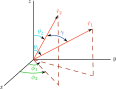
\includegraphics[width=8cm]{Figuras/Addition_Theorem.png}
            \captionof{figure}{Descripción geométrica de los ángulos involucrados en el teorema de adición de armónicos esféricos.}
        \end{center}
       
    
    \end{enumerate}
\end{propiedad}

\begin{ejemplo}
    Dada una partícula cuántica en presencia de un potencial central $V(r)$, su movimiento es descrito por la ecuación de Schrödinger \eqref{eq:schrodinger}, tal que
    \begin{equation*}
        - \frac{\hbar^2}{2m} \left[ \frac{1}{r^2} \frac{\partial}{\partial r} \left( r^2 \frac{\partial}{\partial r} \right) + \frac{1}{r^2 \sin\theta} \frac{\partial}{\partial \theta} \left( \sin \theta \frac{\partial}{\partial \theta} \right) + \frac{1}{r^2 \sin^2\theta} \frac{\partial^2}{\partial \phi^2} + V(r) \right]  \psi = E \psi \ .
    \end{equation*}

    Notemos que, bajo la sustitución
    \begin{equation*}
        k^2 = \frac{2m}{\hbar^2} (V(r) - E) \ ,
    \end{equation*} 
    y reordenando términos, nuestra ecuación puede escribirse como
    \begin{equation*}
        \frac{1}{r^2 \sin\theta} \left[ \sin\theta \frac{\partial}{\partial r} \left( r^2 \frac{\partial}{\partial r} \right) + \frac{\partial}{\partial \theta} \left( \sin \theta \frac{\partial}{\partial \theta} \right) + \frac{1}{\sin\theta} \frac{\partial^2}{\partial \phi^2} + k^2 \right] \psi = 0 \ ,
    \end{equation*}
    lo que corresponde a la ecuación de Helmholtz en coordenadas esféricas \eqref{eq:Helmholtz_esferica}, por lo que al realizar separación de variables, llegaremos a las ecuaciones angulares \eqref{eq:edo_laplace_phi} y \eqref{eq:edo_laplace_theta}. De esta forma, \textbf{para cualquier potencial central}, la componente angular del movimiento tendrá por solución los armónicos esféricos $Y_\ell^m(\theta, \phi)$.
\end{ejemplo}

\begin{ejemplo}
    En mecánica cuántica, puede utilizarse el llamado \emph{formalismo de primera cuantización}, donde se asume que cantidades físicas como posición y momentum corresponden a \emph{operadores} en un espacio vectorial de dimensión infinita. Comúnmente se trabaja en el llamado \emph{espacio de posiciones}, que corresponde al espacio vectorial formado por todos los vectores posición $\x$ en tres dimensiones.
    
    Podemos entender estos operadores como \emph{matrices de dimensión infinita}, por lo que tendrán valores y vectores propios. Sin embargo, los vectores propios no corresponden necesariamente a vectores tuplas, sino que pueden corresponden a \emph{funciones}, pues ellas también son vectores en un espacio vectorial, el \emph{espacio de funciones}.

    El operador \emph{momento angular} se define como un \emph{vector en ``tres dimensiones''}, cuyas componentes pueden escribirse en coordenadas esféricas como
    \begin{align*}
        L_x & = i\hbar \left( \sin \phi \frac{\partial}{\partial \theta} + \frac{\cos \phi}{\tan \theta} \frac{\partial}{\partial \phi} \right) \\
        L_y & = i\hbar \left( -\cos \phi \frac{\partial}{\partial \theta} + \frac{\sin \phi}{\tan \theta} \frac{\partial}{\partial \phi} \right) \\
        L_z & = -i \hbar \frac{\partial}{\partial \phi} \ ,
    \end{align*}
    y su \emph{``operador norma''} se puede escribir como
    \begin{equation*}
        L^2 = -\hbar^2 \left( \frac{\partial^2}{\partial \theta^2} + \frac{1}{\tan \theta} \frac{\partial}{\partial \theta} + \frac{1}{\sin^2  \theta} \frac{\partial^2}{\partial \phi^2} \right) \ .
    \end{equation*}

    En este contexto, es sabido que los operadores $L^2$ y $L_z$ comparten las mismas funciones propias $\psi(r, \theta, \phi)$, de modo que ellas satisfacen 
    \begin{align*}
        L^2 \psi & = -\hbar^2 \left( \frac{\partial^2}{\partial \theta^2} + \frac{1}{\tan \theta} \frac{\partial}{\partial \theta} + \frac{1}{\sin^2  \theta} \frac{\partial^2}{\partial \phi^2} \right) \psi = - \ell(\ell+1) \hbar^2 \psi \\
        L_z & = -i\hbar \frac{\partial \psi}{\partial \phi} = m \hbar \psi \ .
    \end{align*}

    Derivando respecto a $\phi$ la segunda ecuación, tenemos que
    \begin{equation*}
        \frac{\partial^2 \psi}{\partial \phi^2} = i m \frac{\partial \psi}{\partial \phi} = (im) (im) \psi = -m^2 \psi \ ,
    \end{equation*}
    de modo que reemplazando en $L^2 \psi$, tenemos que
    \begin{equation*}
        L^2 \psi - \ell(\ell+1) \hbar^2 \psi = -\hbar^2 \left[ \frac{1}{\sin \theta} \frac{\partial}{\partial \theta}\left( \sin\theta \frac{\partial}{\partial \theta}  \right) + \left( \ell(\ell+1) -  \frac{m^2}{\sin^2 \theta} \right) \right] \psi \ ,
    \end{equation*}
    con lo que nuestro sistema de ecuaciones se ha convertido en las ecuaciones \eqref{eq:edo_laplace_phi} y \eqref{eq:edo_laplace_theta}, cuyas soluciones son los armónicos esféricos. Así, concluímos que las funciones propias comunes a $L^2$ y $L_z$ son los armónicos esféricos, pudiendo escribir que
    \begin{align*}
        L^2 Y_\ell^m(\theta, \phi) & = \ell(\ell+1) \hbar^2 Y_\ell^m(\theta, \phi) \\
        L_z Y_\ell^m(\theta, \phi) & = m \hbar Y_\ell^m(\theta, \phi) \ .
    \end{align*}

    ¿Por qué es útil este hecho? Definiendo los operadores $L_\pm = L_x \pm i L_y$, tendremos que estos satisfacen 
    \begin{equation*}
        L_\pm Y_\ell^m(\theta, \phi) = \hbar \sqrt{\ell(\ell+1) - m(m \pm 1)} Y_\ell^{m \pm 1}(\theta, \phi) \ ,
    \end{equation*}
    por lo que podemos construir una base para las componentes angulares de nuestro espacio vectorial con propiedades bien conocidas, facilitando el estudio del momento angular.
\end{ejemplo}